\documentclass[a4paper]{article}
\usepackage[utf8]{inputenc}
\usepackage[spanish, es-tabla, es-noshorthands]{babel}
\usepackage[table,xcdraw]{xcolor}
\usepackage[a4paper, footnotesep = 1cm, width=20cm, top=2.5cm, height=25cm, textwidth=18cm, textheight=25cm]{geometry}
%\geometry{showframe}

\usepackage{tikz}
\usepackage{amsmath}
\usepackage{amsfonts}
\usepackage{amssymb}
\usepackage{float}
\usepackage{graphicx}
\usepackage{caption}
\usepackage{subcaption}
\usepackage{multicol}
\usepackage{multirow}
\setlength{\doublerulesep}{\arrayrulewidth}
\usepackage{booktabs}

\usepackage{hyperref}
\hypersetup{
    colorlinks=true,
    linkcolor=blue,
    filecolor=magenta,      
    urlcolor=blue,
    citecolor=blue,    
}

\newcommand{\quotes}[1]{``#1''}
\usepackage{array}
\newcolumntype{C}[1]{>{\centering\let\newline\\\arraybackslash\hspace{0pt}}m{#1}}
\usepackage[american]{circuitikz}
\usetikzlibrary{calc}
\usepackage{fancyhdr}
\usepackage{units} 

\graphicspath{{../Calculos-Potencia/}{../Caracteristicas/}{../Consideraciones/}{../Gain-Stage/}{../Input-Stage/}{../Output-Stage/}{../Simulaciones/}{../Alimentacion/}{../Conclusiones/}}

\pagestyle{fancy}
\fancyhf{}
\lhead{22.12 Electrónica II}
\rhead{Mechoulam, Lambertucci, Rodriguez, Londero, Scala}
\rfoot{Página \thepage}

\begin{document}

\tableofcontents
\newpage
\subsection{Diseño Propuesto}
Se requiere una fuente que se ajuste a las siguientes especificaciones:
El cual se ajusta a las especificaciones de:
\begin{align}
0V \leq V_o \leq 9V \ \ \ \ \ \ \wedge \ \ \ \ \ \ I_{o-Max}=2.5A
\end{align} 
Se optó por un diseño que muestre tensión y sume corriente.  
El diseño elegido para la fuente regulada es el siguiente.
\begin{figure}[H]
\centering
	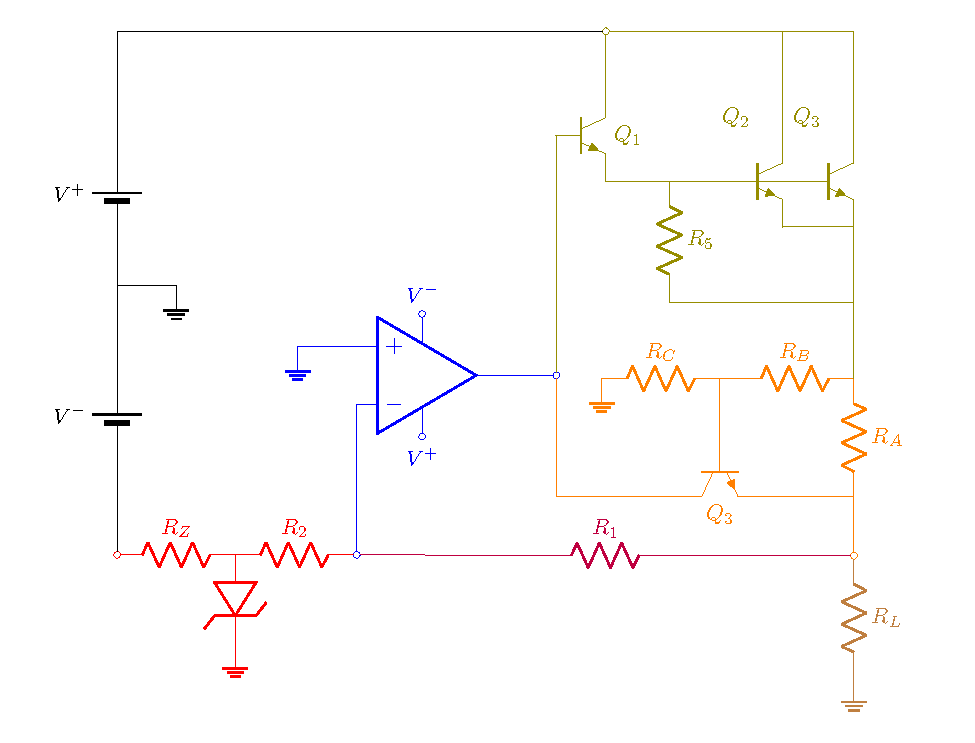
\includegraphics[width=0.8\textwidth, page=1]{ImagenesEjercicio2/Regulador.pdf}
	\caption{Circuito regulador de tensión propuesto.}
	\label{fig:circuitoprop}
\end{figure}
El cual puede ser separado en 5 bloques fundamentales.
\begin{itemize}
\item \textcolor{blue}{Amplificador error}
\item \textcolor{olive}{Transistor de paso}
\item \textcolor{red}{Elemento de referencia}
\item \textcolor{purple}{Circuito de detección}
\item \textcolor{orange}{Circuito de protección}
\end{itemize}

 


\subsubsection{Análisis de realimentación negativa}
\subsubsection{Bloques del Regulador}
\subsubsection{Elemento de Referencia}
\subsubsection{Amplificador de Error y Pre-regulador}
\subsubsection{Circuito de Detección}
\subsubsection{Transistor de Paso}

\subsection{Protección por Corto-circuito}
Implementar una protección de cortocircuito es una sección fundamental en el diseño de una fuente de tensión debido que uno desconoce con que cargas va  a ser utilizado el circuito, en caso de que el usuario en contra-indicación de las especificaciones del equipo utilize una carga menor a la mínima, el circuito no explote. (escribi eso en no mono tomi por favor c:) 
Para la protección de cortocircuito se evaluaron 2 alternativas:
\subsubsection{Protección lineal}
La implementación de una protección lineal resulta ser la mas sencilla debido a la facilidad de cálculo y que utiliza pocos componentes, como se ve a continuación:
\begin{figure}[H]
\centering
	\includegraphics[width=0.5\textwidth, page=3]{ImagenesEjercicio2/Regulador.pdf}
	\caption{Circuito de Protección lineal.}
	\label{fig:circuitolineal}
\end{figure}
El cálculo para la resistencia $R_a= \frac{V_{be}}{I_{o-Max}}$.
Esta protección limita la corriente de salida del regulador haciendola constante. Esto es asi debido a que el trasistor de proteccion sensa la tensión sobre la resistencai $R_a$ y al superar cierto valor $V_a = R_a \cdot I_{o-Max} $ el transistor pasa a modo activo directo, quitandole corriente de la base al transistor de paso.
Si bien la protección lineal es de sencilla implementación cuenta con la siguiente característica:
\begin{figure}[H]
\centering
	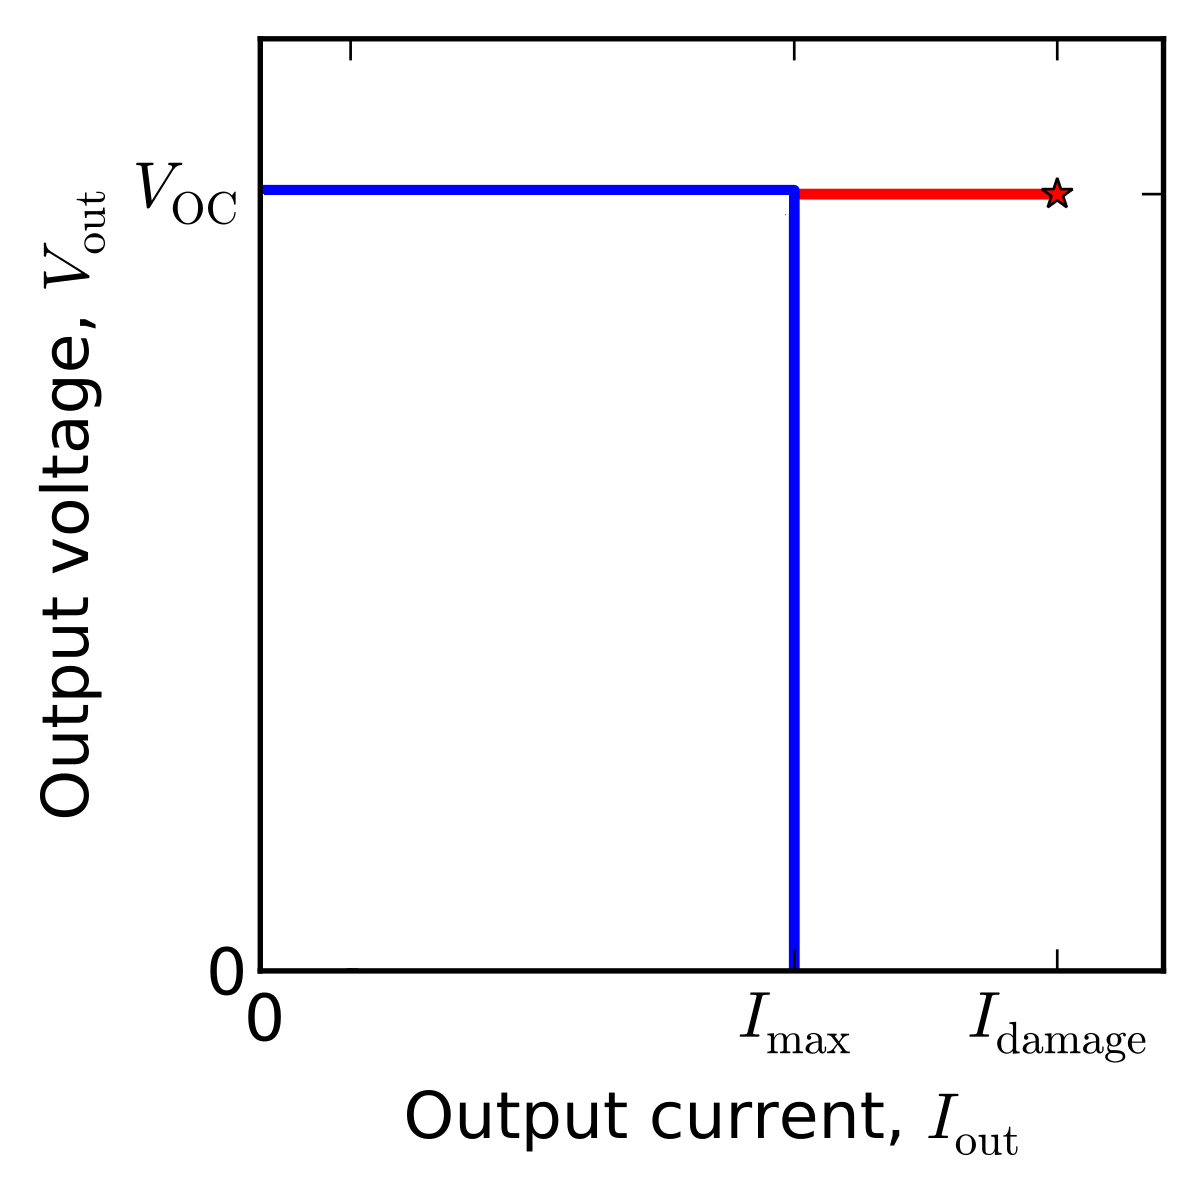
\includegraphics[width=0.5\textwidth]{ImagenesEjercicio2/Linearprotection.png}
	\caption{Característica de la Protección lineal.}
	\label{fig:circuitolinealcarac}
\end{figure}
Se puede notar que en el  peor caso ($V_o = 0$) sería máxima tanto la corriente de salída como la caida de potencail sobre el transistor de paso, haciendo que por consecuente sea máxima la disipación de potencia sobre este, lo cual es un problema.
\subsubsection{Protección foldback}
La protección de Foldback es una variación de la lineal, la cual cuenta con 2 resistencias adicionales conectadas de la siguiente manera:
\begin{figure}[H]
\centering
	\includegraphics[width=0.5\textwidth, page=2]{ImagenesEjercicio2/Regulador.pdf}
	\caption{Circuito de Protección Foldback.}
	\label{fig:circuitofoldback}
\end{figure}
Si se desea resolver para $I_{o-Max}$ bastará con recorrer la malla:
\begin{align}
-I_{o-Max} \cdot R_a + V_{be} - (V_b-V_a)=0
\end{align}
\begin{align}
V_b=V_a \cdot \frac{R_c}{R_c+R_b}
\end{align}
\begin{align}
-I_{o-Max} \cdot R_a + V_{be} + V_a \cdot (1-\frac{R_c}{R_c+R_b})=0
\end{align}
\subsection{Análisis de Componentes}
\subsubsection{Amplificador Operacional}
\subsubsection{Transistores de Paso}
\subsubsection{Componentes de Protección}
\subsubsection{Diodo de Referencia}
\subsubsection{Fuentes de Alimentación}

\subsection{Análisis de Potencia}
\subsubsection{Amplificador Operacional}
\subsubsection{Transistores}

\begin{figure}[H]
\centering
	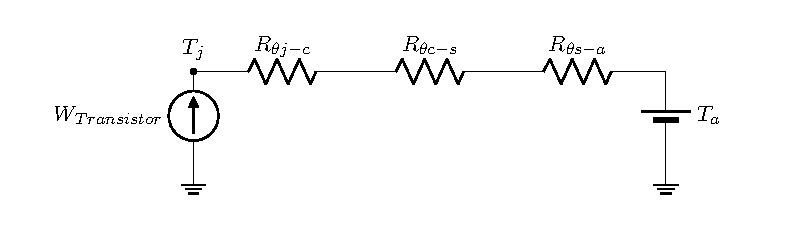
\includegraphics[width=0.6\textwidth, page=1]{ImagenesEjercicio2/Potencia - Transistor.pdf}
	\caption{Circuito térmico para el cálculo de disipador del transistor.}
	\label{fig:circuitopottrans}
\end{figure}

\begin{equation}
\frac{T_j - T_a}{R_{\theta jc}+R_{\theta cs}+R_{\theta sa}} = P
\end{equation}

Asumiendo una temperatura ambiente de $40\degree C$; una temperatura máxima de juntura en funcionamiento de $140\degree C$, $20\degree C$ menor a la especificada por el fabricante; la $R_{\theta jc}$ también especificada, de $3.125\frac{\degree C}{W}$; el uso de una grasa siliconada de 0.002 pulgadas de espesor con una resistencia térmica de $204\frac{\degree C \cdot inch}{W}$, y área estándar de un empaquetado de TO-220 de $0.41\cdot 0.59 inch^2$, obteniendo una $R_{\theta cs}$ de $1.6866 \frac{\degree C}{W}$; y finalmente una potencia disipada de $9.6W$, levemente mayor a la máxima disipada; se obtiene

\begin{equation}
R_{\theta sa} = 4.57 \frac{\degree C}{W}
\end{equation}

\subsubsection{Diodos y Resistencias}

\subsection{Simulaciones}
\subsubsection{Análisis Transitorio en Regulación}
\subsubsection{Respuesta en Frecuencia}
\subsubsection{Curva de Foldback}
\subsubsection{Potencias}

\subsection{Conclusiones}











En la siguiente sección, se busca elaborar una fuente regulada de tensión que cumpla con una salida que varíe entre $0 \ V$ y $9 \ V$, con una corriente de salida máxima de $2.5 \ A$. Dado que la tensión mínima debe ser nula, se implementó un regulador serie que utiliza un lazo de realimentación negativa que muestrea tensión y suma corriente, siendo así el circuito resultante el presentado a continuación.
\begin{figure}[H]
\centering
	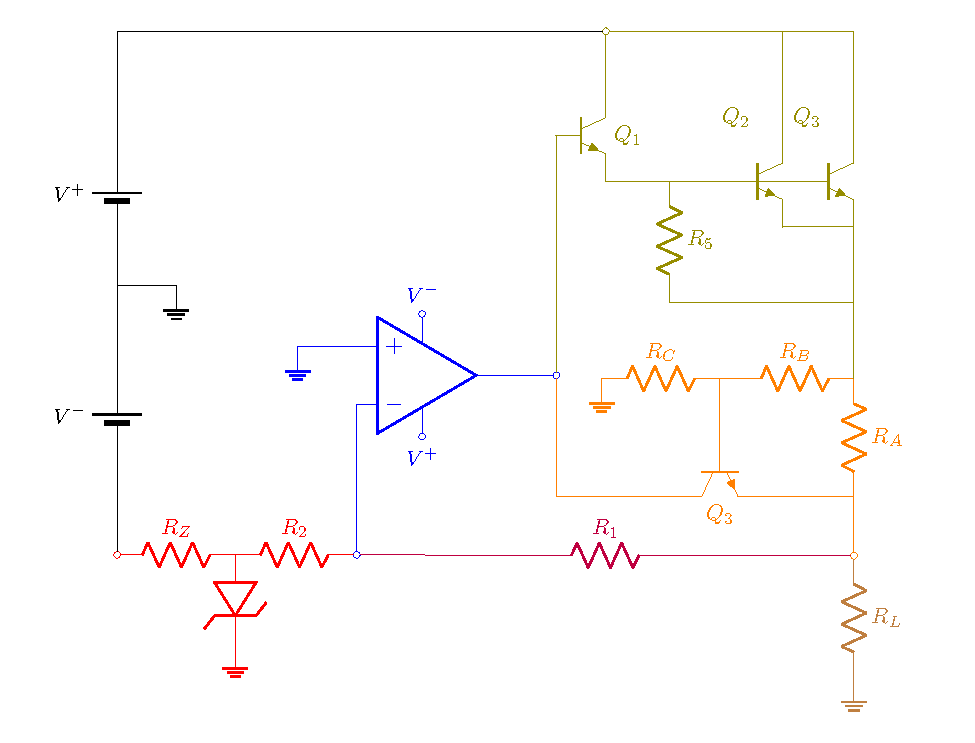
\includegraphics[width=0.8\textwidth, page=1]{ImagenesEjercicio2/Regulador.pdf}
	\caption{Circuito regulador de tensión.}
	\label{fig:circuito1}
\end{figure}

En la Figura (\ref{fig:circuito1}) se puede observar en distintos colores las diferentes etapas del sistema, siendo \textcolor{blue}{en azul el amplificador error}, \textcolor{olive}{en verde el transistor de paso}, \textcolor{red}{en rojo el elemento de referencia}, \textcolor{purple}{en violeta el circuito de detección} y \textcolor{orange}{en naranja el circuito de protección}.

\begin{equation}
\frac{V^- - V_Z}{R_Z} + I_Z = \frac{V_Z}{R_9}
\end{equation}

\begin{equation}
V_{B1max} = V_{Oreg} + V_{Ra} + 1.4 \ V = 9 \ V + 1.25 \ V + 1.4 \ V = 11.65
\end{equation}

\begin{equation}
V_{2min} = 11.65 \ V + 1.5 \ V = 13.15 \ V
\end{equation}

\begin{equation}
	R_{Lmin} = \frac{V_{Omax}}{I_{Omax}} = 3.6 \ \Omega
\end{equation}

\begin{equation}
	R_{Lmax} = \infty
\end{equation}

\begin{equation}
	V_{Lmin} = R_Z \cdot \left( \frac{V_Z}{R_2} + I_z \right) + V_Z
\end{equation}

El pre-regulador cumple la función de brindar corriente \textbf{(habría que desarrollar un poco más)}. Para el caso presente, se observa que el amplificador operacional puede llegar hasta temperaturas de $125 \ ^o C$ son problema. Asumiendo una temperatura ambiente de $40 \ ^o C$, la potencia máxima disipada por operacional es de $0.7 \ W$.
\begin{figure}[H]
\centering
	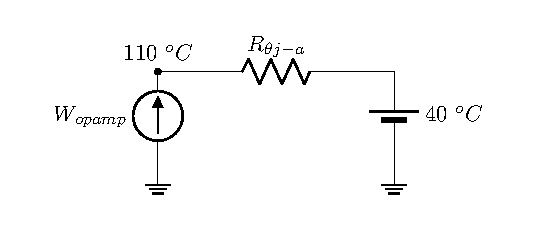
\includegraphics[width=0.6\textwidth, page=1]{ImagenesEjercicio2/Potencia - Opamp.pdf}
	\caption{Circuito equivalente de potencias con $R_{\theta a-j} = 103 \ \frac{^o C}{W}$.}
	\label{fig:circuitopot}
\end{figure}

Es por ello que se analiza la potencia tanto en regulación como fuera de esta. Durante la primer etapa, la tensión de salida $V_O$ es estable pero la corriente es cada vez mayor. A pesar de esto, la potencia disipada por el opamp se mantiene menor a la máxima. Por otro lado, con el circuito fodlback activado, la tensión decae, haciendo que también decaiga la potencia del amplificador, manteniendola por debajo del máximo.
\begin{figure}[H]
\centering
	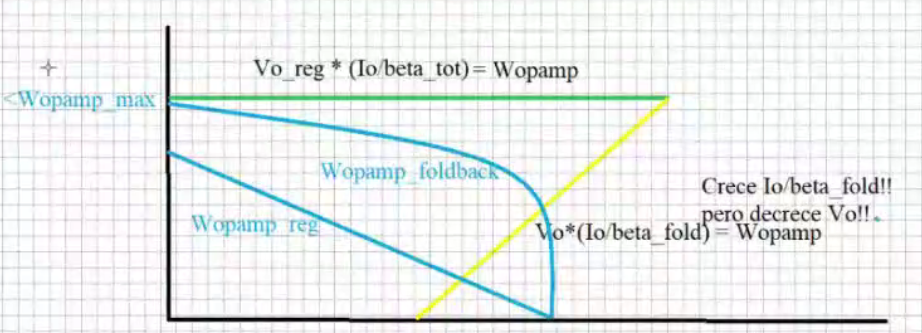
\includegraphics[width=0.6\textwidth]{ImagenesEjercicio2/Potencia2.png}
	\caption{Curvas de potencia consumida.}
	\label{fig:curvapot}
\end{figure}


\end{document}